\chapter{Generación de Mapas a través de RTAB-Map}

En este capítulo se describe el software RTAB-Map, sus características, su proceso de funcionamiento, su instalación y uso en el entorno de desarrollo en sus presentaciones como software independiente o como módulo integrado a ROS y por último, la generación de un mapa de entorno a través del mismo.

\section{Definición}

RTAB-Map (\textit{Real-Time Appearance-Based Mapping} o Cartografía en Tiempo Real Basada en Apariencias) es una aproximación a SLAM mediante Grafo RGB-D basado en un detector de cierre de lazo Bayesiano global. El detector de cierre de lazo usa un modelo de bolsa de palabras para determinar la probabilidad de que una nueva imagen provenga de una ubicación anterior o nueva. Cuando una hipótesis de cierre de lazo es aceptada, una nueva restricción es agregada al grafo del mapa, y un optimizador de grafo minimiza los errores en el mapa. \cite{labbe14online}

Un enfoque de manejo de memoria es utilizado para limitar el número de ubicaciones utilizadas para la detección de cierre de lazos y la optimización del grafo \cite{labbe13appearance}, para que las restricciones de tiempo real en entornos de gran escala sean siempre respetadas. RTAB-Map puede ser utilizado por si solo con un Kinect o cámara estéreo operado a mano para obtener cartografía RGB-D de 6 grados de libertad, o en un robot equipado con un medidor de distancias láser para cartografía de 3 grados de libertad. \cite{rtabmaphome}

La aplicación soporta distintos sensores, tales como el Kinect, el ASUS Xtion Pro / Pro Live \cite{xtionpro} \cite{xtionprolive}, cámaras soportadas por la librería libdc1394 \cite{libdc1394} y cámaras soportadas por la librería FlyCapture2. \cite{libflycapture2}

Como detalle adicional, RTAB-Map permite su uso directamente desde código C++, tanto para detección de cierre de lazos únicamente, como para generar mapas RGB-D.

\section{Instalación}

RTAB-Map soporta instalaciones en Linux, OS X y Windows y puede funcionar de dos maneras: como software independiente (no necesita otros paquetes de software aparte de él mismo y de los controladores de las cámaras a usar) o como un módulo de ROS, en cuyo caso lógicamente requiere que ROS esté instalado de antemano (y la compatibilidad con los distintos sistemas operativos se reduce a la misma de ROS).

\subsection{Como software independiente}

Para instalar el software de forma independiente, tomaremos las instrucciones correspondientes a la instalación en Ubuntu debido a que es el entorno de desarrollo utilizado. Estas instrucciones son tomadas del repositorio del proyecto en Github, a través de la dirección \url{https://github.com/introlab/rtabmap/wiki/Installation}:

\begin{itemize}
	\item Con ROS ya instalado en el sistema:

	Si ya está instalado ROS en el sistema (como es el caso en el desarrollo del proyecto), ya algunas dependencias estarán instaladas:

	Dependencias según versión de ROS:
	Indigo:
	\begin{blackcodebox}
	\begin{lstlisting}[language=bash]
sudo apt-get install libsqlite3-dev libpcl-1.7-all libfreenect-dev libopencv-dev
	\end{lstlisting}
	\end{blackcodebox}
	Hydro:
	\begin{blackcodebox}
	\begin{lstlisting}[language=bash]
sudo apt-get install libsqlite3-dev libpcl-1.7-all ros-hydro-libfreenect ros-hydro-opencv2
	\end{lstlisting}
	\end{blackcodebox}

	Descargue el código fuente de RTAB-Map desde Github:
	\begin{blackcodebox}
	\begin{lstlisting}[language=bash]
git clone https://github.com/introlab/rtabmap.git rtabmap
cd rtabmap/build
cmake ..
make -j4
make install
	\end{lstlisting}
	\end{blackcodebox}

	Ya puede ejecutar la aplicación (llamada ``rtabmap'').

	\item Si ROS no está instalado:

	Dependencias del sistema:
	\begin{blackcodebox}
	\begin{lstlisting}[language=bash]
sudo apt-get install libsqlite3-dev libpcl-1.7-all libopencv-dev
	\end{lstlisting}
	\end{blackcodebox}

	Para instalar libpcl-1.7-all, es posible que deba agregar los repositorios de ROS (en este caso particular, de la distribución de ROS compatible con la distribución de Ubuntu) realizando los siguientes pasos:
	\begin{blackcodebox}
	\begin{lstlisting}[language=bash]
sudo sh -c 'echo "deb http://packages.ros.org/ros/ubuntu $(lsb_release -sc) main" > /etc/apt/sources.list.d/ros-latest.list'
wget http://packages.ros.org/ros.key -O - | sudo apt-key add -
sudo apt-get update
	\end{lstlisting}
	\end{blackcodebox}

	Si desea habilitar las características SURF/SIFT (SURF: \textit{Speeded-Up Robust Features} -- Características Robustas Aceleradas; SIFT: \textit{Scale-Invariant Feature Transform} -- Transformación de Características Invariantes en Escala) en RTAB-Map, deberá descargar y generar OpenCV desde el código fuente para tener acceso al módulo no-libre/privativo:
	\begin{blackcodebox}
	\begin{lstlisting}[language=bash]
cd opencv
mkdir build
cd build
cmake -DCMAKE_BUILD_TYPE=Release ..
make -j4
sudo make install
	\end{lstlisting}
	\end{blackcodebox}

	Descargue el código fuente de RTAB-Map desde Github: obtenga la última versión o el código fuente actual
	\begin{blackcodebox}
	\begin{lstlisting}[language=bash]
git clone https://github.com/introlab/rtabmap.git rtabmap
cd rtabmap/build
cmake ..
make -j4
sudo make install
	\end{lstlisting}
	\end{blackcodebox}

	Ya puede ejecutar la aplicación (llamada ``rtabmap'').

	\item Actualizar el código fuente de RTAB-Map

	Si desea incorporar los últimos cambios después de realizar el ``git clone'' puede actualizarlo de la siguiente forma:
	\begin{blackcodebox}
	\begin{lstlisting}[language=bash]
cd rtabmap
git pull origin master
cd build
cmake ..
make -j4
sudo make install
	\end{lstlisting}
	\end{blackcodebox}
\end{itemize}

\subsection{Como módulo de ROS}

Ubuntu cuenta con binarios para las versiones Hydro e Indigo; basta con ejecutar el siguiente comando, según sea la distribución de ROS:

\noindent ROS Hydro:
\begin{blackcodebox}
\begin{lstlisting}[language=bash]
sudo apt-get install ros-hydro-rtabmap-ros
\end{lstlisting}
\end{blackcodebox}

\noindent ROS Indigo:
\begin{blackcodebox}
\begin{lstlisting}[language=bash]
sudo apt-get install ros-indigo-rtabmap-ros
\end{lstlisting}
\end{blackcodebox}

Si se desea instalar desde fuente, el proceso (detallado en la página \url{https://github.com/introlab/rtabmap_ros#rtabmap_ros}) conlleva tener conocimiento del espacio de trabajo (\textit{workspace}) de ROS, y la instalación desde fuente de la librería OpenCV. También se asume que se ha configurado el espacio de trabajo en el directorio \url{~/catkin_ws} y que el archivo \url{~/.bashrc} contiene lo siguiente:

\noindent ROS Hydro:
\begin{blackcodebox}
\begin{lstlisting}[language=bash]
source /opt/ros/hydro/setup.bash
source ~/catkin_ws/devel/setup.bash
\end{lstlisting}
\end{blackcodebox}

\noindent ROS Indigo:
\begin{blackcodebox}
\begin{lstlisting}[language=bash]
source /opt/ros/indigo/setup.bash
source ~/catkin_ws/devel/setup.bash
\end{lstlisting}
\end{blackcodebox}

Luego, se procede a descargar el código fuente de RTAB-Map desde Github (\textbf{NOTA:} No descargar dentro del espacio de trabajo) e instalarlo dentro del directorio \url{devel} en el espacio de trabajo, ejecutando lo siguiente:
\begin{blackcodebox}
\begin{lstlisting}[language=bash]
cd ~
git clone https://github.com/introlab/rtabmap.git rtabmap
cd rtabmap/build
cmake -DCMAKE_INSTALL_PREFIX=~/catkin_ws/devel ..
make -j4
sudo make install
\end{lstlisting}
\end{blackcodebox}

Ahora puede instalar el ros-pkg de RTAB-Map dentro del directorio \url{src} del espacio de trabajo Catkin:
\begin{blackcodebox}
\begin{lstlisting}[language=bash]
cd ~/catkin_ws
git clone https://github.com/introlab/rtabmap_ros.git src/rtabmap_ros
catkin_make
\end{lstlisting}
\end{blackcodebox}

\section{Generación de Mapas de Entorno}

---Llenar preámbulo---

RTAB-Map comenzará a capturar una nube de puntos en 3D mientras detecta cierres de lazo -- es decir, se lleva a cabo la detección en las ``imágenes'' (ya que no se captura una imagen en sí) de lugares ya visitados previamente, tras lo cual se realizan correcciones en las estimaciones pasadas. Una vez terminado, se puede exportar la nube de puntos capturada a distintos formatos (PCD, que es un formato que contiene datos de nube de puntos \cite{pcdformat} y PLY, que es un formato de polígonos, que guardan datos tridimensionales), para ser procesada posteriormente de ser necesario.

\subsection{Requerimientos}

Para funcionar de forma adecuada, RTAB-Map requiere el uso de las librerías PCL y OpenCV, así como también de los controladores correspondientes al dispositivo que desee usarse, ya sea el Kinect, el Xtion o las múltiples opciones de cámaras estéreo. Asimismo, dependiendo de la configuración del robot y de los sensores disponibles, tendremos múltiples opciones para realizar la cartografía del entorno, todas estas detalladas en la documentación disponible de RTAB-Map, accesible desde el sitio web \url{http://wiki.ros.org/rtabmap_ros/Tutorials/SetupOnYourRobot} (en inglés).

\subsection{Procedimiento y Pruebas}

Con el fin de probar el funcionamiento de RTAB-Map como aplicación independiente e integrada a ROS, seguiremos los tutoriales disponibles en la documentación, primero generando una nube de puntos desde la aplicación independiente, y luego generándola y visualizándola desde ROS.

Cabe destacar nuevamente que, al no contar con un robot propiamente dicho, estaremos utilizando la opción de realizar el mapa únicamente con el Kinect.

\begin{figure}[b]
\centering
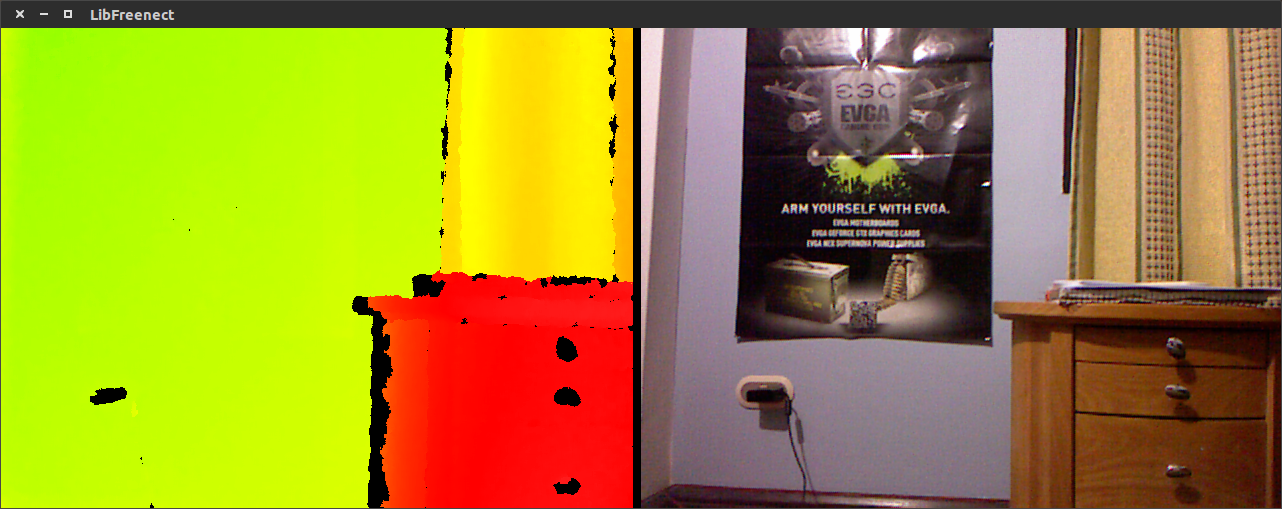
\includegraphics[width=0.75\textwidth]{freenecttest}
\caption{Comprobación de las cámaras del Kinect}
\label{figure:freenecttest}
\end{figure}

Para ello se ha cumplido tanto con la instalación independiente como con la instalación integrada a ROS y se ha comprobado el reconocimiento del Kinect a través del comando:

\begin{blackcodebox}
\begin{lstlisting}[language=bash]
freenect-glview
\end{lstlisting}
\end{blackcodebox}

el cual muestra las imágenes provenientes de ambas cámaras, como se muestra en la figura \ref{figure:freenecttest}

Una vez realizada esta comprobación, podemos continuar con la generación de un mapa de entorno 3D.

\subsubsection{Generación de mapas 3D}

Para esto, realizamos el reconocimiento del entorno a través de la aplicación independiente. Para ello, se inició un terminal y se escribió el comando:

\begin{blackcodebox}
\begin{lstlisting}[language=bash]
rtabmap
\end{lstlisting}
\end{blackcodebox}

cuyo binario está instalado en \url{/usr/local/bin/rtabmap}. Este procedimiento ejecuta el programa, el cual nos pregunta en la primera inicialización, dónde deseamos guardar los datos de la captura (por defecto, esto se realiza en la carpeta \url{/home/<usuario>/Documents/RTAB-Map}).

---Insertar imagen de pregunta---

Tras iniciar, se nos presenta la siguiente pantalla:

---Insertar imagen de pantalla inicial---

Para comenzar la captura de datos de entorno, inicializamos una nueva base de datos haciendo clic en el botón ``New database'':

el cual genera las estructuras de datos necesarias y tras su culminación, estamos listos para realizar la captura. Hacemos clic en el botón Iniciar:

---Insertar imagen de botón iniciar---

Ya podemos comenzar a explorar el entorno. Simplemente basta con dirigir el Kinect haciendo un recorrido del área a obtener, mientras se supervisa la interfaz gráfica de RTAB-Map.

---Insertar imagen de proceso intermedio---

Si en algún momento de la exploración, la pantalla de ``\textit{odometry}'' (odometría) muestra un fondo rojo junto con una imagen estática del entorno, quiere decir que no se tienen suficientes características distintivas en la zona capturada para poder realizar una medición adecuada. Para arreglarlo, tal como se nos indica en el tutorial correspondiente, debemos colocar la cámara de nuevo en la zona que se muestra en la imagen y esperar a que la aplicación retome la generación del mapa desde ese punto.

Una vez explorado el área, hacemos clic en el botón ``Stop'', tras lo cual podemos examinar los resultados, presentados en la figura \ref{figure:bedroommap}.

\begin{figure}[hb]
\centering
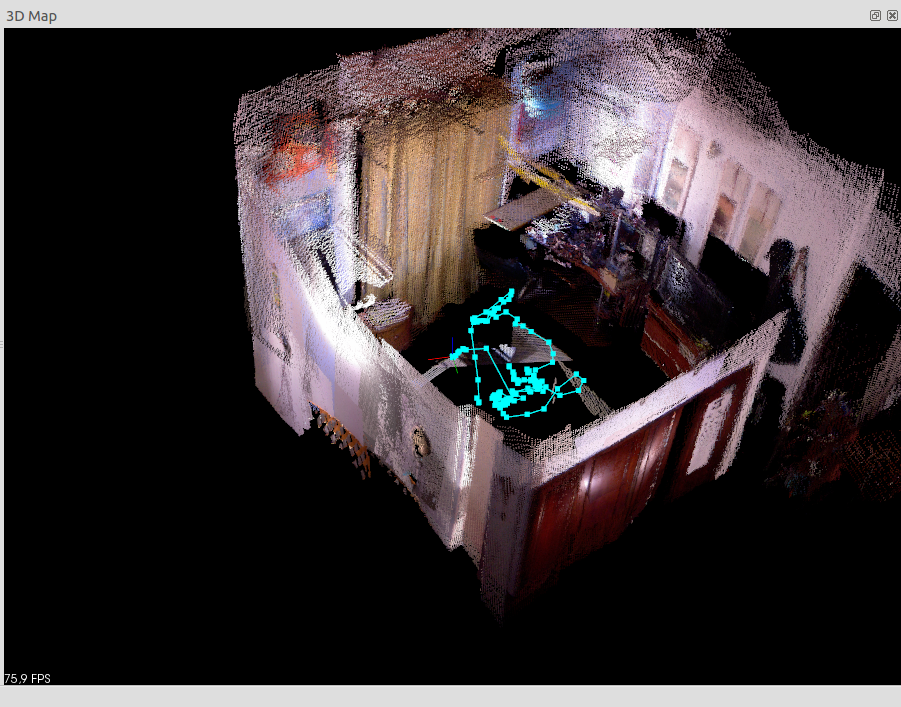
\includegraphics[width=1.00\textwidth]{bedroommap}
\caption{Generación de nube de puntos de una habitación}
\label{figure:bedroommap}
\end{figure}

En el mapa 3D generado, se puede observar una serie de puntos en cian conectados entre sí, que representan la trayectoria de la cámara (en este caso, del Kinect), al generar el mapa.

\subsubsection{Generación de mapas 2D}

La generación de un mapa 2D no es sino la proyección en el plano de la nube de puntos capturada en el paso anterior. Para esto, utilizaremos la versión de RTAB-Map integrada a ROS, ya que por inconvenientes al momento de instalar la versión independiente, no se reconoce de forma adecuada la librería PCL, necesaria para generar la ``rejilla de ocupación'' (en inglés, ``\textit{occupancy grid}'') que sería el mapa en 2D de los obstáculos detectados durante la generación del mapa.

Procedemos de la siguiente forma:

En primer lugar, requeriremos el uso del software de control para el Turtlebot \cite{turtlebot}, que es un kit robótico de bajo costo. Este software permite simular un robot y provee de archivos de lanzamiento adecuados para nuestro caso de uso. Se instala mediante el siguiente comando:

\begin{blackcodebox}
\begin{lstlisting}[language=bash]
sudo apt-get install ros-indigo-turtlebot ros-indigo-turtlebot-apps ros-indigo-turtlebot-interactions ros-indigo-turtlebot-simulator ros-indigo-kobuki-ftdi ros-indigo-rocon-remocon ros-indigo-rocon-qt-library ros-indigo-ar-track-alvar-msgs
\end{lstlisting}
\end{blackcodebox}

Una vez instalado, debemos agregar dos archivos de lanzamiento particulares al directorio de instalación de Turtlebot en ROS, disponibles en el repositorio en Github del proyecto de RTAB-Map en la dirección \url{https://github.com/introlab/rtabmap_ros/}, ejecutando los siguientes comandos en una terminal:

\begin{blackcodebox}
\begin{lstlisting}[language=bash]
sudo wget -P /opt/ros/indigo/share/rtabmap_ros/launch/demo/ https://raw.githubusercontent.com/introlab/rtabmap_ros/master/launch/demo/demo_turtlebot_mapping.launch
sudo wget -P /opt/ros/indigo/share/rtabmap_ros/launch/demo/ https://raw.githubusercontent.com/introlab/rtabmap_ros/master/launch/demo/demo_turtlebot_rviz.launch
\end{lstlisting}
\end{blackcodebox}

Una vez terminadas las descargas, debemos ejecutar cada uno de estos comandos en una terminal independiente:

\begin{blackcodebox}
\begin{lstlisting}[language=bash]

\end{lstlisting}
\end{blackcodebox}

\begin{blackcodebox}
\begin{lstlisting}[language=bash]

\end{lstlisting}
\end{blackcodebox}

\begin{blackcodebox}
\begin{lstlisting}[language=bash]

\end{lstlisting}
\end{blackcodebox}

Este último comando inicia la herramienta RViz, o Visualizador de ROS, el cual permite obtener datos de distintos nodos y tópicos disponibles.

---Insertar imagen de RViz---



---Llenar.---

\paragraph{Selección de altura máxima para generación del mapa 2D}

---Llenar.---